\let\cleardoublepage\clearpage
\chapter{System Overview}
\begin{figure}[!htb]
\centering
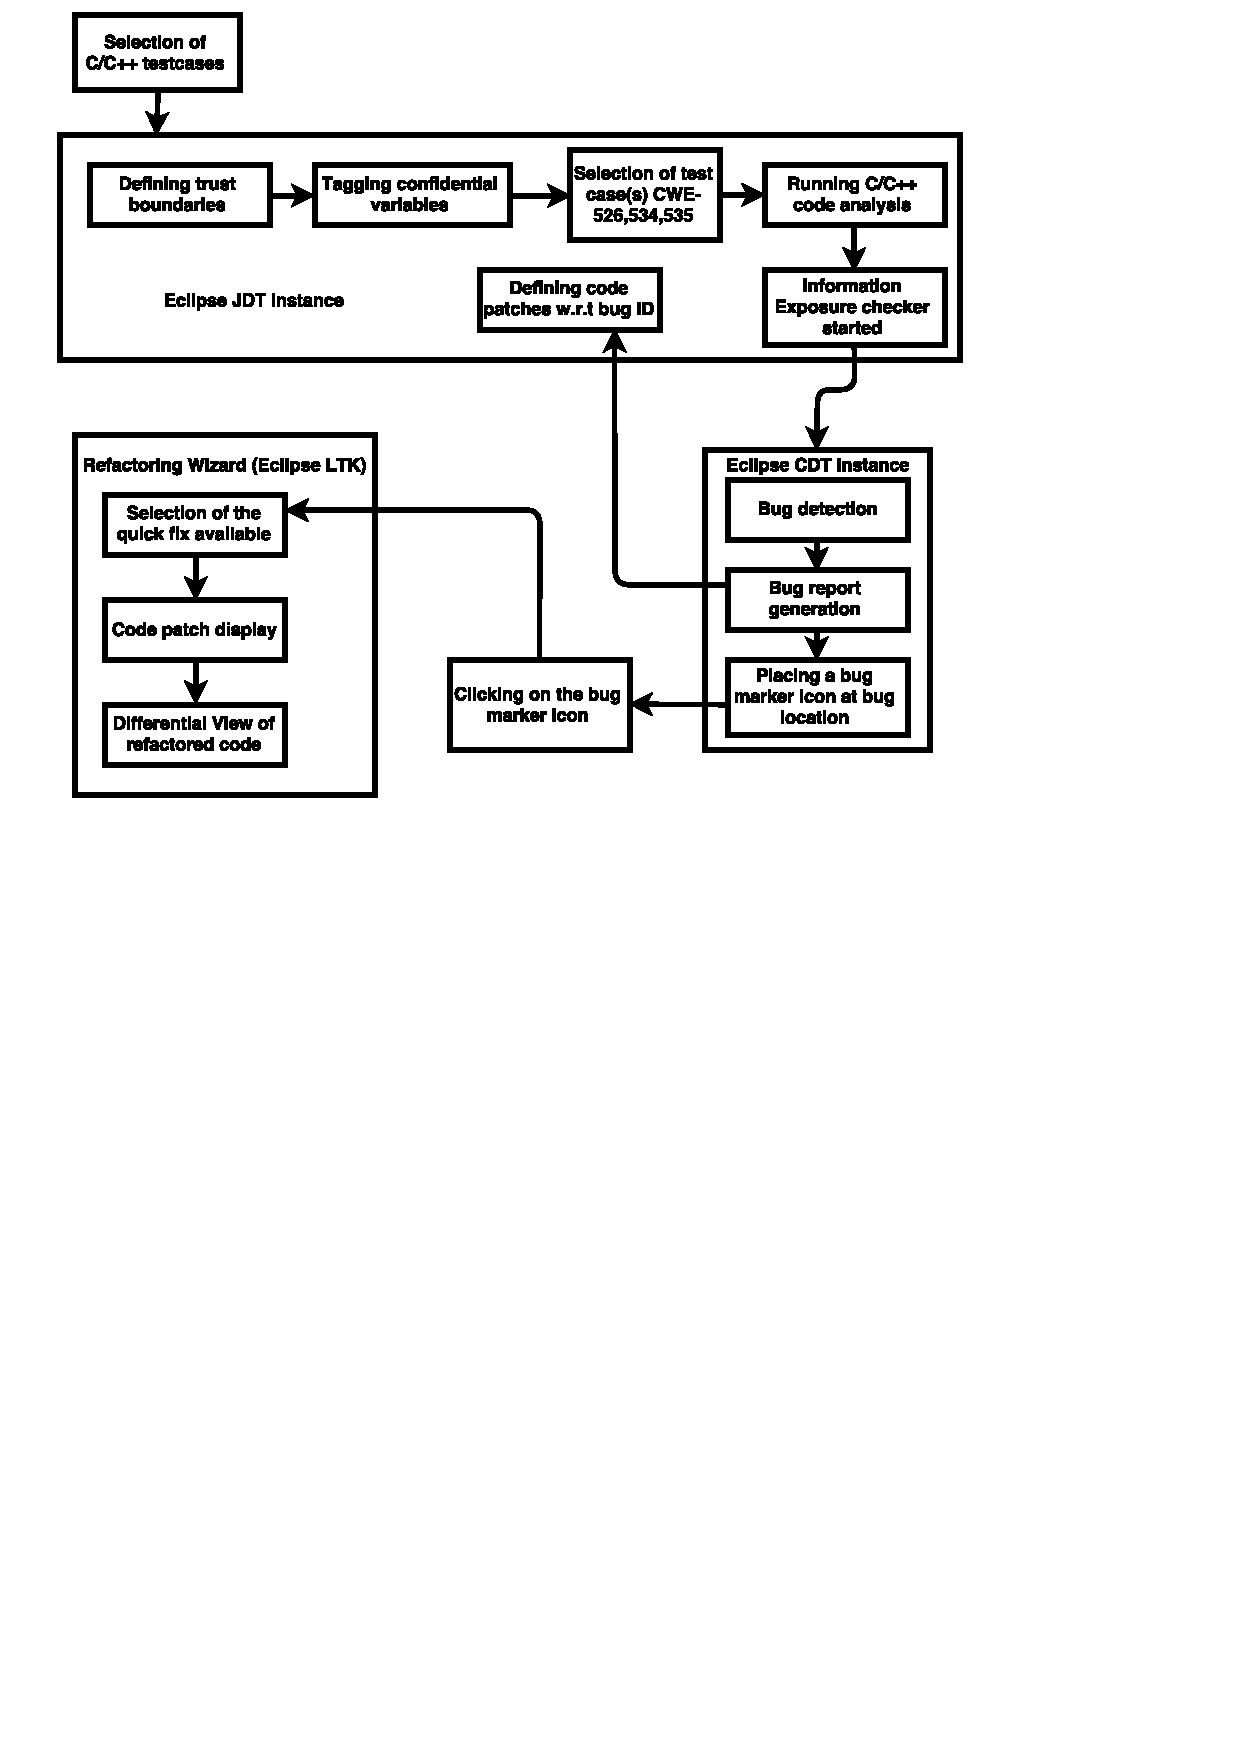
\includegraphics[trim=0.0cm 0.0cm 0.0cm 0.0cm, scale=0.9]{pdf/system.pdf}
\vspace{-15.5cm}
\caption{System Overview}
\label{fig:system}
\end{figure}
Exisiting information-flow checker is based on the static analysis engine
which can be scaled to many other types of checkers and also for large 
test cases. The system workflow is depicted in figure~\ref{fig:system}.
Step by step procedure involved in the system's workflow:
\begin{itemize}
 \item  all the C/C++ test programs have to be selected which are to be imported
in the workspace.
\item  all the confidential variables in the test
programs have to be tainted and the trust boundaries need to be defined.
\item  after running the eclipse java application, a new eclipse CDT instance
is launched in which we can find already imported test programs.
\item then a test
program is selected and a sub menu "Run C/C++ Code Analysis" option
has to selected after right clicking on it.
\item a refactoring wizard
appears after clicking on the bug marker that is placed after running the
information exposure checker.
\end{itemize}

Basically the IE checker is run as an Eclipse
plug-in project. Once this project is started a new eclipse CDT instance is 
launched as shown in the figure~\ref{fig:tool1} containing 90 Test Programs(TP)
namely CWE-526, CWE-534, CWE-535. A Graphical User Interface(GUI) is provided by the codan API.
After running the checker the results can be seen in the view represented
by figure~\ref{fig:tool2}. We can also use one of the Codan API feature in order
to configure the bug report's representation to be Warnings, errors or infos.
The end result of the IF checker is the bug report containing the description
of the bug, the file and the path which can lead to the location of the bug on 
clicking
on the warning message as represented in figure~\ref{fig:tool2} marked with number 3.
After reaching the bug location in the file, upon clicking on the bug marker icon
a refactoring wizard is launched containing the quick fix options as shown in 
figure~\ref{fig:tool4}. After selecting any one option, a window with the selected
code patch is displayed and upon clicking next,differential view with
both the buggy program and refactored code is displayed as shown in 
figure~\ref{fig:tool6}. After clicking on finish the code is refactored.



\label{chapter:Algorithm}

\chapter{Localization Algorithm}
\label{chapter:Algorithm}
{\LinesNumberedHidden
\begin{algorithm}
\caption{Decision on starting the localization algorithm for searching quick fix locations and for generating the code patches}
\label{alg:one}
\SetAlgoLined
\KwIn{$location_{node}$, $filename_{node}$,$sourcefile_{node}$}

\KwOut{Refactorings set $R_{set}:=$ \{$r_j\arrowvert$ 0 $\leq$ j $\textless$ 2 \}} 

$N_{set}:=$ \{$n_t\arrowvert$ 0 $\leq$ t $\leq$ n,$\forall$ n $\geq$ 0 \};       \textcolor{dkgreen}{\textbf{\fontfamily{cmtt}\selectfont{//set of nodes}}}\\
$R_{set}:$=$\emptyset$;$N_{set}:$=$\emptyset$\;        \textcolor{dkgreen}{\textbf{\fontfamily{cmtt}\selectfont{//initialising nodes set and refactoring set to empty}}}\\
$j=0$;

\underline{function CheckerReport} $(location_{node}, filename_{node}, sourcefile_{node})$

\eIf {$filename_{node}\neq sourcefile_{node}$}
{
$localizer.start()$;          \textcolor{dkgreen}{\textbf{\fontfamily{cmtt}\selectfont{//Starting the localizer}}}\\
}
{
$N_{set}:=N_{set}\bigcup{node}$;     \textcolor{dkgreen}{\textbf{\fontfamily{cmtt}\selectfont{//adding node to node set}}}\\
$r_{j}:= refact(node)$;       \textcolor{dkgreen}{\textbf{\fontfamily{cmtt}\selectfont{//Refactoring the node}}}\\
$R_{set}:=R_{set}\bigcup{r_{j}}$;      \textcolor{dkgreen}{\textbf{\fontfamily{cmtt}\selectfont{//adding refactored node}}}\\
$j=:j+1$\;
}
\end{algorithm}
}

Alogrithm~\ref{alg:one} explains how the decision is made for running the localizer
algortihm. The input for this algorithm is the node containing the bug location,
filename and also the source code file name. Output is a set of refactorings.
For the current test programs we find a set of two refactorings only.
First we initialise the nodes set $node_{set}$, refactorings set $R_{set}$ to empty set.
Then, after the IE checker reports a bug a check is done in order to find if the
file in which the bug was detected is a source file or not. If both the file name and the source files
are not the same then the localizer is started else refactorings for the detected
buggy nodes is done. In the process of refactoring the nodes, the buggy nodes
are collected and then manual code patches for the coressponding bugs are made. Then 
the manually made code patches are then translated into nodes and with
the help of eclipse LTK the code patches are then inserted into the buggy program.


{\LinesNumberedHidden
\begin{algorithm}[ht]
\caption{Part-I: Localizer algorithm and generating code patches}
\label{alg:two}
\SetAlgoLined
\KwIn{Set of satisfiable paths $Sat_{paths}:=$\{$spath_i\arrowvert$ 0 $\leq$ i $\leq$ n,$\forall$ n $\geq$ 0 \};}

\KwOut{Refactorings set $R_{set}:=$ \{$r_j\arrowvert$ 0 $\leq$ j $\textless$ 2 \}} 
$N_{set}:=$ \{$n_t\arrowvert$ 0 $\leq$ t $\leq$ n,$\forall$ n $\geq$ 0 \};     \textcolor{dkgreen}{\textbf{\fontfamily{cmtt}\selectfont{//Set of Nodes}}}\\
$pathloc_{list}:=$ \{$path_k\arrowvert$ 0 $\leq$ k $\leq$ n,$\forall$ n $\geq$ 0 \};     \textcolor{dkgreen}{\textbf{\fontfamily{cmtt}\selectfont{//Set of paths list with filename and line number of every node in the path}}}\\
$path_{location}:$=$\emptyset$;      \textcolor{dkgreen}{\textbf{\fontfamily{cmtt}\selectfont{//list of nodes in the path with filename and linenumber}}}\\
$R_{set}:$=$\emptyset$;       \textcolor{dkgreen}{\textbf{\fontfamily{cmtt}\selectfont{// initialising refactorings set}}}\\
$N_{set}:$=$\emptyset$;       \textcolor{dkgreen}{\textbf{\fontfamily{cmtt}\selectfont{// initialising nodes set}}}\\

\underline{function Localizer} $()$

\While{(($Sat_{paths}$.hasNext))}{
\For{\textbf{each} $node_{j}$ \textbf{in} $spath_{i}$}{
 \eIf{$node_{j}.hasTranslationalUnit()$}{
 $filename:=node_{j}.getfilename()$\;
 $linenumber:=node_{j}.getStartingLinenumber()$\;
}{
 $filename:=null$\;
 $linenumber:=-1$\;
 }
 $path_{location}:=path_{location}\bigcup getloc(filename,linenumber)$;     \textcolor{dkgreen}{\textbf{\fontfamily{cmtt}\selectfont{//Add location of each node in the path}}}\\
  }
  $pathloc_{list}:=pathloc_{list}\bigcup path_{location} $;      \textcolor{dkgreen}{\textbf{\fontfamily{cmtt}\selectfont{//Updating the paths list}}}\\
  \For{\textbf{each} $buginfo$ \textbf{in} $spath_{i}$}{         \textcolor{dkgreen}{\textbf{\fontfamily{cmtt}\selectfont{//verifying if the path has the bug info}}}\\
  $bugloc_{new}:=bugloc(path_{location})$\;
  $loc_{bugloc}:=loc_{bugloc}\bigcup bugloc_{new} $;         \textcolor{dkgreen}{\textbf{\fontfamily{cmtt}\selectfont{//Updating the localizer bug locations}}}\\
  }
    $path_{location}:$=$\emptyset$;       \textcolor{dkgreen}{\textbf{\fontfamily{cmtt}\selectfont{//emptyping the pathlocation}}}\\
}
\For{\textbf{each} $bugloc$ \textbf{in} $loc_{bugloc}$}{
\For{$i \gets 1$ \textbf{to} $bugloc.pathdepth$ }{       \textcolor{dkgreen}{\textbf{\fontfamily{cmtt}\selectfont{//we count the number of times the node appears in the buggy paths}}}\\
\eIf{$node_{i}$ \textbf{in} $path_location$ of $loc_{bugloc}$ }{
$count:=count+1$;         \textcolor{dkgreen}{\textbf{\fontfamily{cmtt}\selectfont{//Updating the count of the node}}}\\
}
{
$count:=0$;         \textcolor{dkgreen}{\textbf{\fontfamily{cmtt}\selectfont{//Updating count to 0 if it appears for the first time}}}\\
}

}
$bugmap:=bugmap.buginfo.put(node_{i},count)$;         \textcolor{dkgreen}{\textbf{\fontfamily{cmtt}\selectfont{//maintaing a map between the node and its count}}}\\
}
\begin{algorithmic}                   % enter the algorithmic environment
\STATE
\algstore{myalg}
\end{algorithmic}
\end{algorithm}
}

{\LinesNumberedHidden
\begin{algorithm}[ht]
\caption{Part-II Localizer algorithm and generating code patches}
\begin{algorithmic}                   % enter the algorithmic environment
\algrestore{myalg}
\STATE
\end{algorithmic}
\For{\textbf{each} $buginfo$ \textbf{in} $bugmap$}{
\For{\textbf{each} $path_{k}$ \textbf{in} $pathloc_{list}$}{
\For{\textbf{each} $path_{l}$ \textbf{in} $loc_{bugloc}$}{
\eIf{$path_{k} \neq path_{l}$}{
          \textcolor{dkgreen}{\textbf{\fontfamily{cmtt}\selectfont{// remove all definitely good nodes (from paths without the bug) and
			nodes without a useful location }}}\\
$bugmap.remove(path_{k})$\;
}
{
continue;
}
}
}
}
\For{\textbf{each} $node$ \textbf{in} $bugmap$}{
          \textcolor{dkgreen}{\textbf{\fontfamily{cmtt}\selectfont{// Get the node with the maximum count}}}\\
\If{$node.getcount()> max$}{$max:=node.getcount()$}
\If{$node.getcount()= max$}{
$suspicious_{node}:=suspicious_{node} \bigcup node$;      \textcolor{dkgreen}{\textbf{\fontfamily{cmtt}\selectfont{// 
node with max count is the suspicious node}}}\\
$node_{map}:= node_{map} \bigcup getpath(node)$;          \textcolor{dkgreen}{\textbf{\fontfamily{cmtt}\selectfont{// 
save the node and its corresponding path in a hashmap}}}\\
}
\eIf{$node_{map}.size \le 1$}{
$N_{set}:=N_{set}\bigcup{node}$;       \textcolor{dkgreen}{\textbf{\fontfamily{cmtt}\selectfont{//adding node to node set}}}\\
$r_{j}:= refact(node)$;         \textcolor{dkgreen}{\textbf{\fontfamily{cmtt}\selectfont{//Refactoring the node}}}\\
$R_{set}:=R_{set}\bigcup{r_{j}}$;          \textcolor{dkgreen}{\textbf{\fontfamily{cmtt}\selectfont{//adding refactored node}}}\\
$j=:j+1$\;
}{          \textcolor{dkgreen}{\textbf{\fontfamily{cmtt}\selectfont{//if nodes belong to same path then find first node 
in the path}}}\\
\eIf{$node in node_{map} belong to same path$}{
$N_{set}:=N_{set}\bigcup{firstnode}$;        \textcolor{dkgreen}{\textbf{\fontfamily{cmtt}\selectfont{//adding node to node set}}}\\
$r_{j}:= refact(node)$;          \textcolor{dkgreen}{\textbf{\fontfamily{cmtt}\selectfont{//Refactoring the node}}}\\
$R_{set}:=R_{set}\bigcup{r_{j}}$;        \textcolor{dkgreen}{\textbf{\fontfamily{cmtt}\selectfont{//adding refactored node}}}\\
$j=:j+1$\;
}{             \textcolor{dkgreen}{\textbf{\fontfamily{cmtt}\selectfont{//if nodes belong to different paths create refactoring for each node
in different paths}}}\\
$N_{set}:=N_{set}\bigcup{node}$;         \textcolor{dkgreen}{\textbf{\fontfamily{cmtt}\selectfont{//adding node to node set}}}\\
$r_{j}:= refact(node)$;                \textcolor{dkgreen}{\textbf{\fontfamily{cmtt}\selectfont{//Refactoring the node}}}\\
$R_{set}:=R_{set}\bigcup{r_{j}}$;         \textcolor{dkgreen}{\textbf{\fontfamily{cmtt}\selectfont{//adding refactored node}}}\\
$j=:j+1$\;
}
}
}
\end{algorithm}
}




Algorithm~\ref{alg:two} shows how a localizer works. Input for this algorithm is a set 
of satisfiable paths $Sat_{paths} $ and output is a set of refactorings $R_{set}$.
$N_{set}$ is the set of nodes. $pathloc_{list}$ is a set of paths list which contains
the nodes which inturn contains the file name and the line number of every node in 
a particular path. Initially $pathloc_{list}$, $R_{set}$, $N_{set}$ are all set to empty.
Below are the steps followed in the localizer algorithm:
\begin{itemize}
 \item First the localizer checks for the satisfiable paths.
 \item For every node in the path it then checks if the node has a translation unit using the 
 the function \emph{hasTranslationalUnit()}.
 \item If the node has a translational unit then the filename and the linenumber
 of that particular node is stored else the value of the filename is set to null and 
 the line number to be -1. 
 \item Particular node values are then added to the $path_{location}$ set.
 \item Once all the nodes in a particular path has been traversed and its filename and
 linenumber are stored then the particular path details are added to the $pathloc_{list}$
 set. This is done until all the satisfiable paths exist.
 \item Then the frequency of the nodes occuring in all the satisfiable paths is counted.
 \item Once all the nodes frequency is counted, then all the nodes with their respective
 frequency is maintained in a bugmap data structure.
 \item Now all the not buggy paths are removed form the list of all satisfiable paths in a way
 that all the nodes which appeared in both the buggy and not buggy paths are also removed.
 This makes sure that the nodes that appear in both buggy and not buggy path are
 not the cause for the bug. In this way one can filter out the not suspicious nodes.
 \item Filtering helps us to save time when we start back traversing the paths in order
 to find the "not-in-place" quick fix locations. 
 \item Once all the not buggy nodes are removed from the bugmap then we check for the
 node which contains the maximum frequency. The node which contains the maximum
 frequency is supposed to be the most suspicious node. If we have nodes with the same
 frequency then all the nodes are collected and added to the set of $suspicious_{nodes}$
 and also the path of that coressponding node in $node_{map}$ hashmap.
 \item We then check the size of the $node_{map}$, if the $node_{map}$ size is 1 then 
 the refactoring is created for that particular node and added to the refactorings list.
 \item If the size of $node_{map}$ is greater than one then we check if the nodes 
 in the hashmap belong to different program paths.
 \item If the nodes belong to different program paths then the refactoring for 
 every suspicious node is created and added to the set of refactorings node.
 \item If they doesnot belong to different nodes then the earliest node
 that appears in the program execution path is considered to be the 
 earliest quick fix location and a refactoring for only that node is created and added
 to the refactorings list.
 
 
 After all the refactorings are created then the generated code patches are 
 then inserted
 into the buggy program with the help of eclipse LTK API, in order to remove the bugs.
 This localizer is very efficient and faster in localising the bugs. Detecting the "not 
-in-place" fix can also ne done by backward propagation of all the nodes in the 
buggy path butit takes more time then the localizer because in localizer
we donot parse all the nodes. We filter the not suspicious nodes and 
parse only the suspicious nodes. Therefore we happen to parse very less number
of nodes using the localizer then backward propagation mechanism. Figure~\ref{fig:localizer}
depicts the activity diagram of the localizer and how the decisions are made.
In the eclipse LTK API that has been used with show two types of options
at the time of refactorting i.e, "Earliest Fix" and "Latest Fix" which means the
"not-in-place" fix and the "in-place" fix respectively. In the test program CWE-526
we use the localizer because the bug was detected initially at one of the library files.
Therefore one cannot insert or change any code in the library files because
there can be many other function which make use of those library files. So in order to
avoid this we made use of the localizer to find a location where the bug can be
fixed in the source file itself but not in the library files.
 
\end{itemize}

\begin{figure}[!htb]
\centering
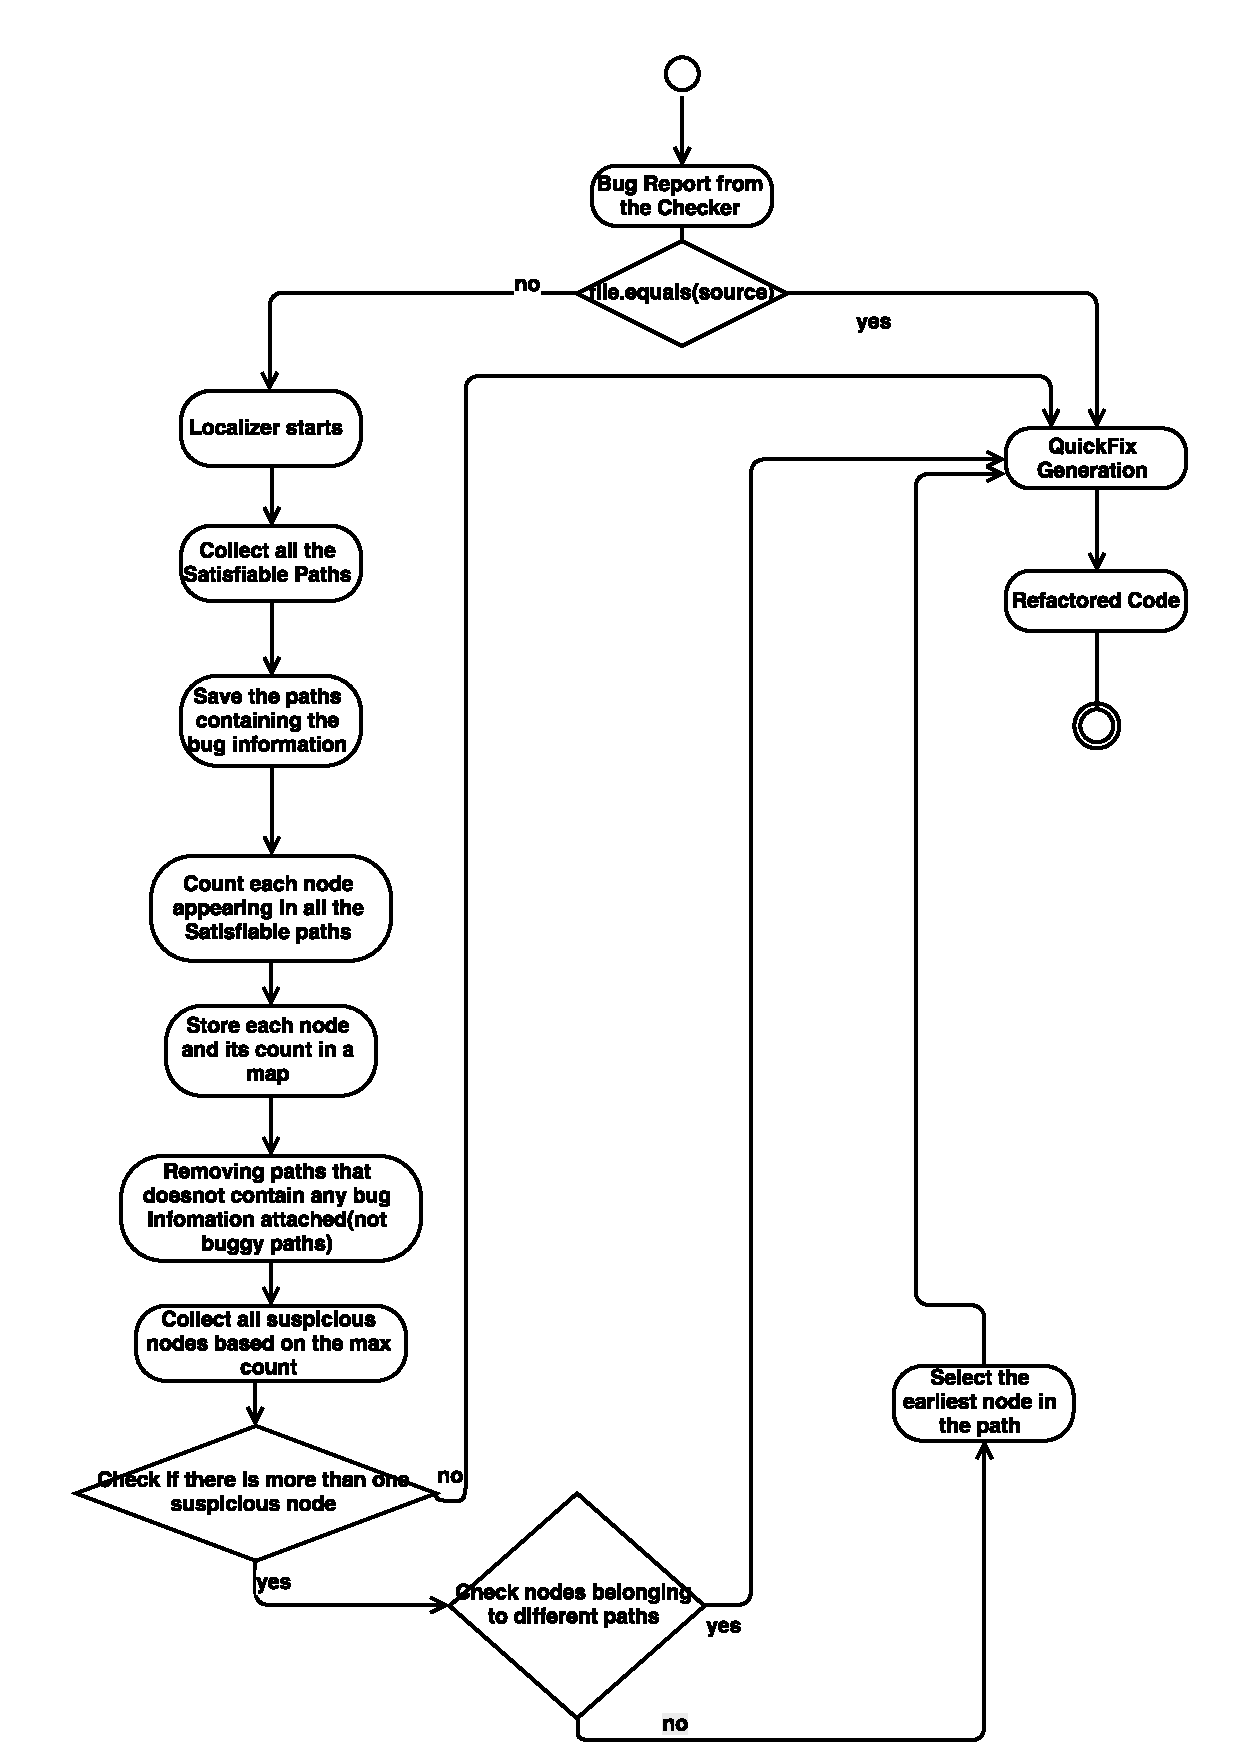
\includegraphics[trim=0.0cm 0.0cm 0.0cm 0.0cm, scale=0.75]{pdf/Localizer.pdf}
\vspace{-0.5cm}
\caption{Localizer activity diagram}
\label{fig:localizer}
\end{figure}

\chapter{Approach}
\label{chapter:Approach}

General Steps involved in detecting, localizing and fixing bugs are:
\begin{itemize}
 \item Identifying the error
 \item Finding the error
 \item Analyzing the error
 \item Proving the analysis
 \item Covering all the lateral damages
 \item Fixing the error
 \item Validating the solution
\end{itemize}

\textbf{Identifying the error:} This is a general step in which we
identify the error. There are times when some errors can waste a lot
of our developing time. Sometimes the errors reported by the users are also
hard to interprete and some of the information could also be misleading.
Therefore one can do the following steps:
\begin{itemize}
 \item See the error if it is understandable or ask the user to send some screenshots.
 \item Try to reproduce the error. One should not claim that there is no error
 without reproducing it.
 \item Understanding the expected behaviour. In some of the complex applications
 ,it is difficult to understand the expected behaviour of an error. So, it is better
  to ask the product owner or check the documentation in order to find the
  expected behaviour of the error.
  \end{itemize}
  
  
\textbf{Finding the error:} Once we have indentified the error, we then have to 
find where the error is located. One has to go through the code in order to find
the error location. Imagine if there thousand lines of code it is very diffcult
to go through the code. Some of the techniques that could be helpful are:
\begin{itemize}
 \item Logging
 \item Debugging
 \item Removing code
\end{itemize}


\textbf{Analyzing the error:} This step is a bottom-up approach in which
we try to analyze the code from the place we found the error and try to figure 
out the cause for the error.

\textbf{Proving the Analysis:} After analyzing the error, there
might be some other errors influenced by the original error. so 
one has to come up with some automated test cases.


\textbf{Covering lateral damage:} At this step the developer
would be ready with the code patch that he wanted to insert
into the code in order to remove the error but he should
be careful enough that the original behaviour of the program
is not at all disturbed.


\textbf{Fixing the error:} Finally after all the verfication
for program behavior to be preserved is done, we then
insert the code patch in order to fix the bug.


\textbf{Validating the solution:} Once again we run all the
test cases in order to make sure that the error is removed.



Therefore all these steps can be handled manually for softwares
which contain very less number of lines of code. Imagine
a large project where there are thousands of lines of code.
It is really a hetic task to identify and fix the bugs.
In order to make this task simpler we need to automate the
process. The aim of this thesis is to provide a tool for this
process of fixing the errors automatically.




\section{About the Tool}
Developed tool bridges the gap between the bug report 
that is been reported by the already exisitng information
exposure bug checker and the automatically generated one
or more bug fixes which helps in the removal of the information
exposure bugs. Removal of the bug is tested again by re-running
the information exposure checker on the patched program.
Bug fixes includes 
structure of the fix, location where the fix has 
to be inserted
and the values used in the fix patches. The bug localization
for some files is done
by the information exposure checker which is 
integrated in our static analysis engine and
by the localizer for other files which contain 
the wrapper functions. The checker basically returns the file name,
line number and also a bug ID which is unique for every kind of bug.
Therefore along with the report, the checker also puts a marker at the bug location.
After clicking the icon the refactoring wizard starts.


\section{Bug Detection with tainting and triggering}

Function models were used in order to describe the behaviour of the C/C++ library function calls.
Static analysis engine's implementation is dependant on these function models.
Every function model class will contains five methods and also it implements the IFctModel.
The methods are: the constructor, \emph{getName()} used for returning the function name,
\emph{getLibrarySignature()} for returning the whole header of that function 
same as it is in the C standard library defined, \emph{exec(SymFunctionCall call)}
used for executing the function calls statically
in which the variables can be tainted and also the trust
boundaries are defined which could help
in notifying the checker, \emph{getSignature()} used for returning a SymFctSignature object
which contains the data types of the parameters of that particular function call
and also the return type of the function itself.
Major difference between \emph{exec()} method of the 
function models \emph{printf()} and getenv is that the IF
checker is notified that a trust-boundary is about to be passed
in \emph{printf()} function model and in \emph{getenv()} the return type of the \emph{exec()}
method is set to be confidential. In the same way the source and sink 
which are contained in CWE-534/CWE-535 are implemented.


\begin{lstlisting}[caption={Function model of getenv()},label={lst:getenv()}]


	public Mgetenv(Interpreter ps) {
		this.ps = ps;
		HashMap<String, Comment> commentMap = AnnotationExecution
				.getCommentsMap();
		if (commentMap == null) {
			MyLogger.log_parser("Comment Map is Empty");
		} else {
			comment = commentMap.get(getLibrarySignature());
			if (comment == null) {
				MyLogger.log_parser("Mgetenv comment is null");
			} else {

				if (comment.getType().equals(Comment.singleLineComment)) {
					annotationType = Comment.singleLineComment;
					listSingleParamterAnnotation = AnnotationParserUtil
							.getSingleLineParamterAnnotation(comment);
					listSingleFunctionAnnotation = AnnotationParserUtil
							.getSingleLineFunctionAnnotation(comment);
					if (listSingleParamterAnnotation == null) {
					} else {
					}
				} else if (comment.getType()
						.equals(Comment.mutilineLineComment)) {
					annotationType = Comment.mutilineLineComment;
					listMultiParamterAnnotation = AnnotationParserUtil
							.getMultilineParameterComment(comment);
					listMultiFunctionAnnotation = AnnotationParserUtil
							.getMultilineFunctionComment(comment);
				}
			}
		}
	}

	public String getName() {
		return "getenv";
	}

	private static String getLibrarySignature() {
		return "extern char *getenv (__const char *__name) __THROW __nonnull ((1)) __wur;";
	}

	public SymFunctionReturn exec(SymFunctionCall call) {
		ArrayList<IName> plist = call.getParams();
		SymPointerOrig isp = ps.getLocalOrigSymPointer(plist.get(0));
		IName nebn = new EnvVarName();
		SymIntOrig sb_size = new SymIntOrig(new ImpVarName());
		SymArrayOrig sb = new SymArrayOrig(nebn, sb_size);
		try {
			sb.setElemType(eSymType.SymPointer);
			SymVarSSA ssa = (SymVarSSA) ps.declareLocal(eSymType.SymPointer,
					null);
			isp_ssa = (SymPointerSSA) ps.ssaCopy(isp);
			isp_ssa.setTargetType(eSymType.SymPointer);

			if (comment != null && annotationType != null
					&& annotationType.equals(Comment.mutilineLineComment)
					&& listMultiFunctionAnnotation != null
					&& listMultiParamterAnnotation != null) {
				String function_property = AnnotationUtil.FUNCTION_PROPERTY_SOURCE;
				if (listMultiFunctionAnnotation.get(0).getAtribute()
						.equals(function_property.toString())) {
					
					if (listMultiParamterAnnotation.get(0).getIndex() == 0) {
						String security_level = AnnotationUtil.PARAMTER_SECURITY_LEVEL_CONFIDENTIAL;
						if (listMultiParamterAnnotation.get(0)
								.getSecurityType()
								.equals(security_level.toString())) {
							isp_ssa.setConfidential(true);
						} else {
							isp_ssa.setConfidential(false);
						}
					}
				} else {
				}
			}
			isp_ssa.setTarget(sb);
		} catch (Exception e) {
			e.printStackTrace();
		}
		return new SymFunctionReturn(isp_ssa);
	}

	public SymFctSignature getSignature() {
		SymFctSignature fsign = new SymFctSignature();
		fsign.addParam(new SymPointerOrig(eSymType.SymArray, new Integer(1)));

		fsign.setRType(new SymPointerOrig(eSymType.SymPointer, new Integer(1)));
		return fsign;
	}

}
\end{lstlisting}

\begin{lstlisting}[caption={Function model of printf()},label={lst:printf()}]

	public Mprintf(Interpreter ps) {
		this.ps = ps;

		commentMap = AnnotationExecution.getCommentsMap();
		if (commentMap == null) {
			MyLogger.log_parser("Comment Map is Empty");
		} else {
			comment = commentMap.get(getLibrarySignature());
			if (comment == null) {
				MyLogger.log_parser("Mgetenv comment is null");
			} else {

				if (comment.getType().equals(Comment.singleLineComment)) {
					annotationType = Comment.singleLineComment;
					listSingleParamterAnnotation = AnnotationParserUtil
							.getSingleLineParamterAnnotation(comment);
					listSingleFunctionAnnotation = AnnotationParserUtil
							.getSingleLineFunctionAnnotation(comment);
					if (listSingleParamterAnnotation == null) {
					} else {
					}
				} else if (comment.getType()
						.equals(Comment.mutilineLineComment)) {
					annotationType = Comment.mutilineLineComment;
					listMultiParamterAnnotation = AnnotationParserUtil
							.getMultilineParameterComment(comment);
					listMultiFunctionAnnotation = AnnotationParserUtil
							.getMultilineFunctionComment(comment);
				}
			}
		}
	}

	public String getName() {
		return "printf";
	}

	public static String getLibrarySignature() {
		// contained in stdio.h
		return "extern int printf (__const char *__restrict __format, ...);";
	}

	public SymFunctionReturn exec(SymFunctionCall call) {
		ArrayList<IName> plist = call.getParams();
		SymArraySSA newdestarr = null;
		SymArraySSA sourcearr = null;
		try {
			int t = 0;
			t = plist.size() - 1;
			
			SymVarSSA sourceSSA = (SymVarSSA) ps
					.resolveOrigSymVar(plist.get(t)).getCurrentSSACopy();

			if (sourceSSA != null && comment != null && annotationType != null) {
				
				if (annotationType.equals(Comment.mutilineLineComment)
						&& listMultiFunctionAnnotation != null
						&& listMultiParamterAnnotation != null) {
					String function_property = AnnotationUtil.FUNCTION_PROPERTY_SINK;
					for (FunctionComment element : listMultiFunctionAnnotation)
						if (element.getAtribute().equals(
								function_property.toString())) {
							ps.notifyTrustBoundary(sourceSSA);
						} else {
						}
				} else {
				}
			}
		} catch (Exception e) {
			e.printStackTrace();
		}
		IName retname = new ImpVarName();
		SymPointerOrig retvalorig = new SymPointerOrig(retname);
		retvalorig.setTargetType(eSymType.SymPointer);
		SymVarSSA ssa = (SymVarSSA) ps.declareLocal(eSymType.SymInt, null);
		return new SymFunctionReturn(ssa);
	}
	public SymFctSignature getSignature() {
		SymFctSignature fsign = new SymFctSignature();
		fsign.addParam(new SymPointerOrig(eSymType.SymArray, new Integer(1)));
		fsign.addParam(new SymPointerOrig(eSymType.SymArray, new Integer(1)));

		fsign.setRType(new SymPointerOrig(eSymType.SymPointer, new Integer(1)));
		return fsign;
	}

}
\end{lstlisting}


Function model that currently exists in SAE are some of the C functions:
\emph{atoi()}, \emph{fclose()}, \emph{fgets()}, \emph{fwgets()},
\emph{fgetws()}, \emph{fopen()}, \emph{gets()}, \emph{memcpy()}, \emph{mod()},
\emph{puts()}, \emph{rand()}, \emph{srand()}, \emph{strcpy()}, \emph{strlen()},
\emph{time()}, \emph{wcscpy()}, \emph{wcslen()}.
Funtion models which were used in this thesis are \emph{getenv()}
as the source and \emph{printf()} as the sink from the test programs CWE-526.
\emph{LogonUserA()}, \emph{LogonUserW()} as source and \emph{fprintf()}, \emph{fwprintf()} as sink
from the test programs CWE-534 and CWE-535.
These function models were used for both tainting and also triggering.



\section{Semi Automated Patch insertion Wizard}
\label{semi:insert}
The information exposure checker after detecting a bug, it places
a bug marker which is a yellow color bug icon
as shown in the figure~\ref{fig:tool3}. It is placed to the left side
of the C/C++ statement at the place where it contains a information
exposure bug. Therefore, after clicking on the bug marker, one
can start the wizard for the code refactoring. This wizard
contains three user pages. In the first page, the user can make
a selection of either "in-place" (latest) or
"not-in-place" (earliest) fixes as shown in figure~\ref{fig:tool4}.  
In the second page one can have a look at the code patch that
is going to be inserted in the code for refactoring as shown in figure~\ref{fig:tool5}. In the third
page one can have a differential view depicting the 
difference between the refactored code and the original 
source code files as shown in figure~\ref{fig:tool6}. One can navigate through all the three pages 
using the buttons "Back", "Next", "Cancel" in order to see the 
changes inserting "in-place" and "not-in-place" fixes.
Finally, once the decision has been made on the selection
user has to click on "finish" button in order to make sure that
the selected patch is written to the file and then the wizard 
exits.

\section{Tool Demo}
\label{demo:behavior}
The refactoring process is carried out stepwise. Following windows shows all the steps involved:\\
1. After running the Eclipse Java application, a CDT instance is displayed. From this
instance one can select a testcase that are imported from the Juilet testsuite as shown in figure
~\ref{fig:tool1}.
After the selection of testcase, right click on the testcase. Once clicked,
a window with many options appear. Among the options click on "Run C/C++" Code Analysis.
Once the analysis is run then the Information Exposure checker is started and checks for
the bugs.\\
\begin{figure}[!htb]
\centering
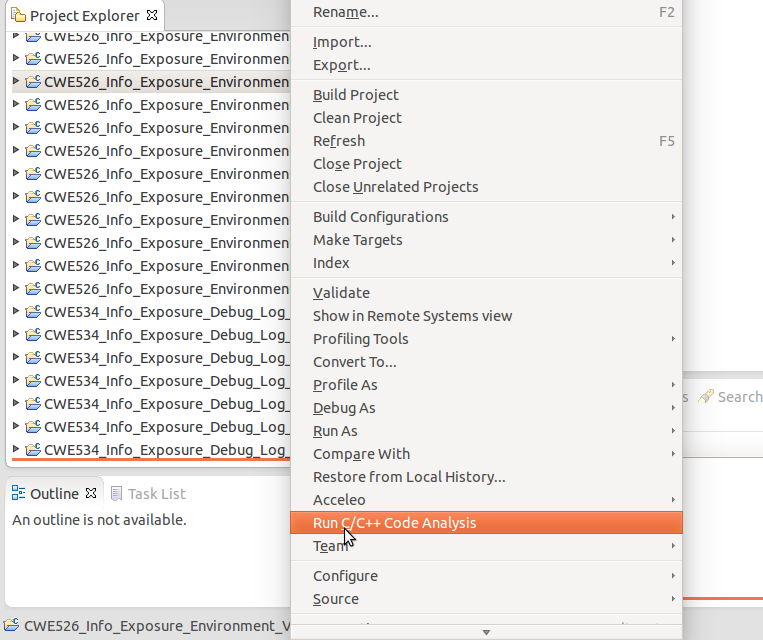
\includegraphics[width=0.9\textwidth]{png/Tool1.png}
\caption{C/C++ testcase selection and running analysis}
\label{fig:tool1}
\end{figure}\\
2. After the checker checks for the information exposure bugs. The next window consists of three views: A view
with yellow color
marker placed at the location where the bug was detected as shown in the figure~\ref{fig:tool2} annotated 
with \textbf{2}. A view displaying all the bugs that are found, annotated with \textbf{3} and by clicking on 
any of the bug details in the window, it takes us to the location where the bug is located. A view with the the list
of all the testcases annotated with \textbf{1}\\
\begin{figure}[!htb]
\centering
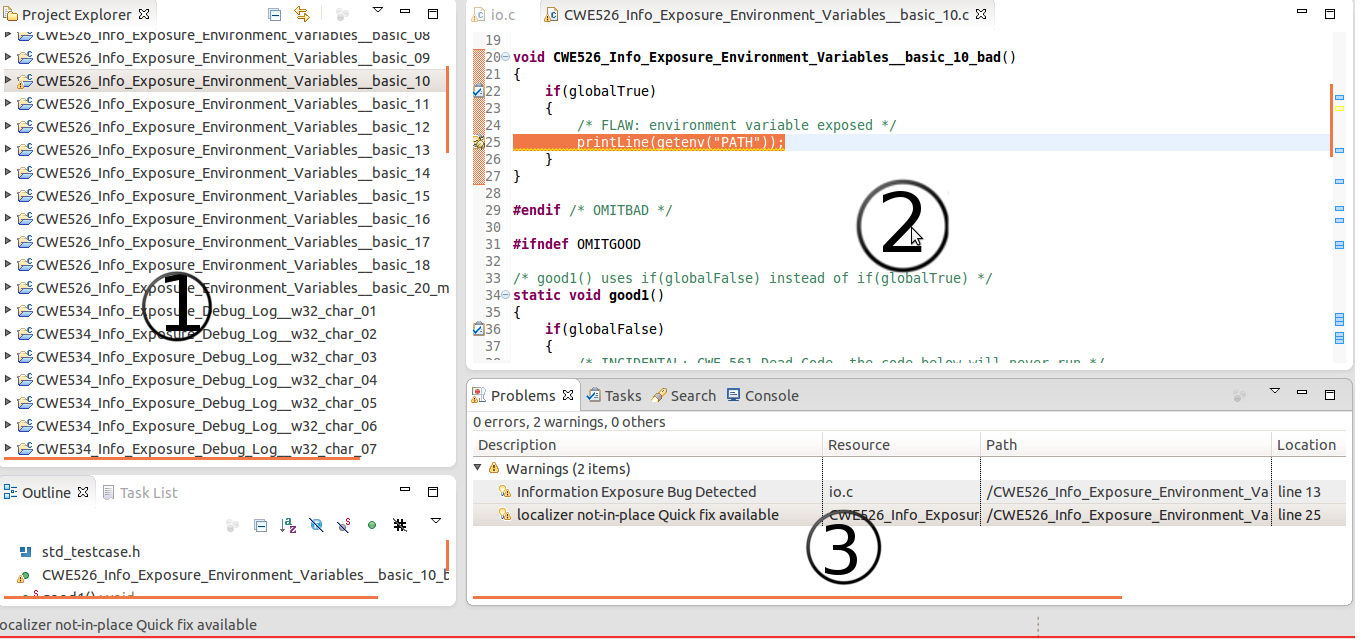
\includegraphics[width=1.0\textwidth]{png/Tool2.png}
\caption{Marker at the bug location}
\label{fig:tool2}
\end{figure}\\
3. When a user places the mouse cursor on the yellow icon which is the bug marker. A small window with a message 
the problem message and description is displayed as shown in the figure~\ref{fig:tool3} e.g "Quick fix is available"
and "Problem description: localizer not-in-place Quick fix available"\\
\begin{figure}[!htb]
\centering
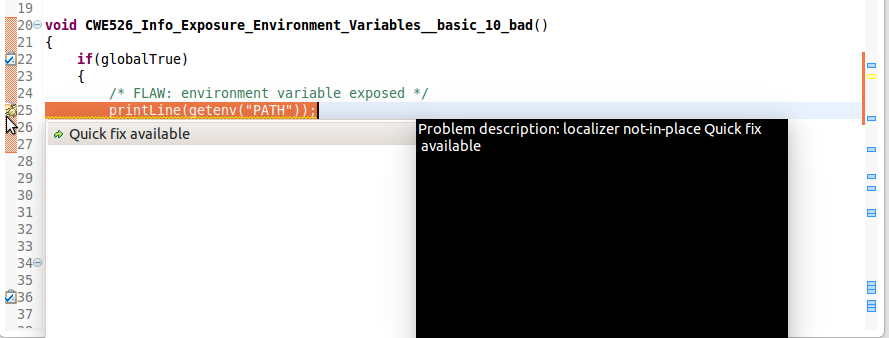
\includegraphics[width=1.0\textwidth]{png/Tool3.png}
\caption{Click on the marker icon}
\label{fig:tool3}
\end{figure}\\
4. After clicking on this bug marker icon a window showing the following option is displayed with
earliest quick fix(not-in-place) and latest quick fix(in-place). After selecting any one of the option
and clicking on "Next" button will take the user to the next window. By clicking on the "Cancel" button
will stop the refactoring process as shown in figure~\ref{fig:tool4}.\\
\begin{figure}[!htb]
\centering
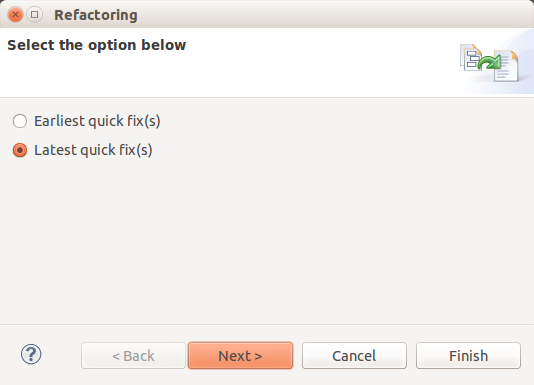
\includegraphics[width=0.7\textwidth]{png/Tool4.png}
\caption{Refactoring Wizard with two options}
\label{fig:tool4}
\end{figure}\\
5. User can then see a window which displays the code patch based on the selection in the previous
window . Here "printLine("Confidential data has been restricted")" is the code patch. User can go 
to the previous window by clicking on "Back" button, "Finish" to proceed to the next window, `
"Cancel" to cancel the refactoring process as shown in figure~\ref{fig:tool5}.\\
\begin{figure}[!htb]
\centering
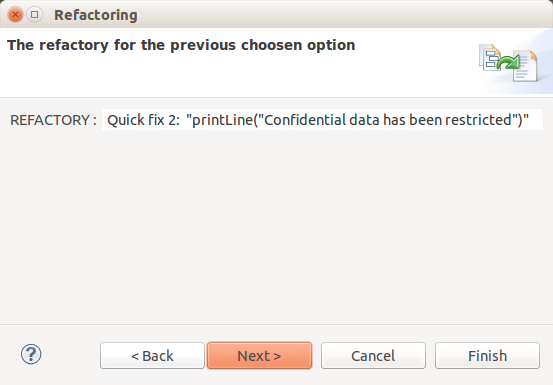
\includegraphics[width=0.7\textwidth]{png/Tool5.png}
\caption{Patch according to the previous selection}
\label{fig:tool5}
\end{figure}\\
6. Once the user clicks on "Next" from the previous window figure~\ref{fig:tool5}, then a 
window with differential view is displayed which shows the difference between the original code
and the refactored code by highlighting the place where the code was refactored as shown in figure~\ref{fig:tool6}.\\
\begin{figure}[!htb]
\centering
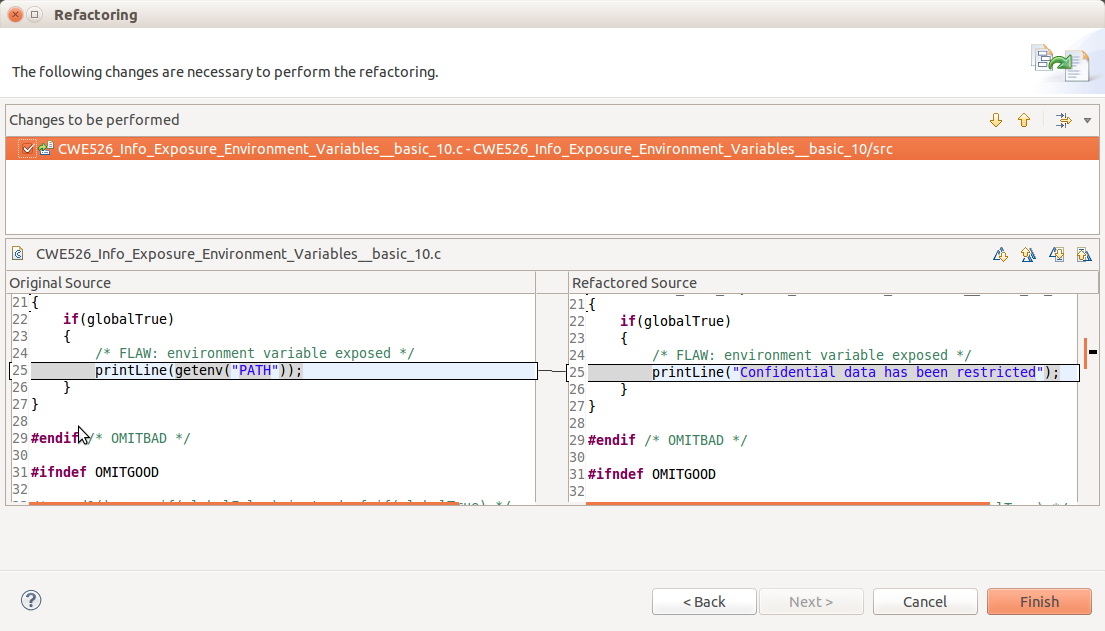
\includegraphics[width=1.0\textwidth]{png/Tool6.png}
\caption{Differential view of the patched and unpatched programs}
\label{fig:tool6}
\end{figure}\\
 
\chapter{Implementation}
\label{chapter:impl}


Developed information exposure bugs fixing tool was integrated into already existing Static Analysis Engine(SAE) which
is a plugin of Eclipse IDE. A Refactoring wizard was developed in order to semi-automatically insert the generated code patch
into the buggy program in order to fix the errors. This was developed using the Eclipse Language Tool Kit (LTK), JFace and 
CDT. Refactoring of code is done in two steps: First, performing bug detection analysis where if the bug was found
a marker icon is placed at the bug location. This is the "in-place" location. If the marker is put in a file other than
the original source code file then we start the localization algorithm. This is because, other files may contain
wrapper functions where the bug was detected but we cannot fix the bug at that location since this
wrapper function may be used by other functions where there is no confidential data being sent. Therefore,
we have to fix the bug at 
a place in the source code file from where the confidential data leaves. This is the "not-in-place" fix location.
So after running the localizer algorithm we get some suspicious nodes. From these 
suspicious nodes, we then again propagate
through all the nodes in order to verify if some confidential 
information flows through it. This can be done
by checking it the variables are tagged with the tag "confidential". Once we find the exact node from where
 the information started flowing, again a marker is placed at that location. Once the bug fix locations are found, then 
 we start the refactoring wizard in order to insert the code patches into the buggy code.
This refactoring LTK API is found in org.eclipse.ltk.core.refactoring and org.eclipse.ltk.ui.refactoring 
plug-ins. 

In general the life cycle of a refactoring is as follows:
\begin{itemize}
 \item First the user starts refactoring.
 \item Verfication is done to see if the refactoring is applicable at that
 context as desired by the user using the function \emph{checkInitialCondtions()}
 \item If necessary, the user is asked if he has additional information.
 \item Once all the information is available then a final check is performed
 using \emph{checkFinalConditions()} and all the changes in their
 source text are calculated using \emph{createChange()}.
 \item After this the differential view with both the source code and
 the refactored code appears and once the user clicks on OK then the
 refactoring is done.
 \end{itemize}
 
 \emph{org.eclipse.ltk.core.refactoring.Refactoring} subclass should always 
 be created which is the main class for the refactorting. For the 
 refactoring participants to be supported \emph{ProcessorBasedRefactoring}
 should be extended. And also a subclass of org.eclipse.ltk.ui.refactoring.RefactoringWizard
 is necessary for the UI side which is used for handling every
 individual pages of the refactoring wizard through which the
 user will be able to scroll with the help of "next" and "back" and also
 "finish" in order to invoke the final operation of the refactoring
 process.
 
 
 Steps followed for refactoring:
 \begin{itemize}
  \item In the first step when all the information required for 
  triggering the refactoring is collected. For example consider
  that the plug-in has a text selection, therefore the information
  about the selected text and also its position in the 
  document is saved in an info object. So this info object is then
  evaluated with the help of RenamePropertyRefactoring.
  \begin{lstlisting}[caption={Class RenameProperty},label={lst:refac}]
RefactoringProcessor processor = new RenamePropertyProcessor( info );
RenamePropertyRefactoring ref = new RenamePropertyRefactoring( processor ); 
RenamePropertyWizard wizard = new RenamePropertyWizard( ref, info );
RefactoringWizardOpenOperation op = new RefactoringWizardOpenOperation(wizard ); 
try { 
	String titleForFailedChecks = ""; //$NON-NLS-1$ 
	op.run(getShell(), titleForFailedChecks ); 
} catch( InterruptedException irex ) { 
	// operation was cancelled 
}
  \end{lstlisting}

  \item Now LTK controls the next process. Initially the \emph{checkInitialCondtions()}
method is called on the refactoring object. This checks if the
basic conditions are enough for the refactoring. 

  \begin{lstlisting}[caption={Class RenamePropertyDelegate},label={lst:refacDel}]

RefactoringStatus checkInitialConditions() {
	RefactoringStatus result = new RefactoringStatus();
	IFile sourceFile = info.getSourceFile();
	if( sourceFile == null || !sourceFile.exists() ) {
		result.addFatalError( CoreTexts.renamePropertyDelegate_noSourceFile );
	} else if( info.getSourceFile().isReadOnly() ) {
		result.addFatalError( CoreTexts.renamePropertyDelegate_roFile );
	} else if( isEmpty( info.getOldName() ) || !isPropertyKey( info.getSourceFile(), info.getOldName() ) ) {
		result.addFatalError( CoreTexts.renamePropertyDelegate_noPropertyKey );
	}
	return result;
}
\end{lstlisting}

\item Once the result from the above step is satisfied then
the wizard is displayed and asks the user for additional information
if necessary. This UI is implemented as a subclass of \emph{UserInputWizardPage}
Whichever the data has been entered at this point is then
made available to the \emph{RenamePropertyRefactoring} via the
Info object.
\item \emph{checkFinalConditions()} method is called before the
last page is displayed via the refactoring wizard. All the changes
are then handled by the createChange() method.

  \begin{lstlisting}[caption={Class RenamePropertyDelegate(core)},label={lst:refacDel}]
private Change createRenameChange() {
	// create a change object for the file that contains the property
	// which the user has selected to rename
	IFile file = info.getSourceFile();
	TextFileChange result = new TextFileChange( file.getName(), file );
	// a file change contains a tree of edits, first add the root of them
	MultiTextEdit fileChangeRootEdit = new MultiTextEdit();
	result.setEdit( fileChangeRootEdit );
	
	// edit object for the text replacement in the file, this is the only child
	ReplaceEdit edit = new ReplaceEdit( info.getOffset(),
	info.getOldName().length(),
	info.getNewName() );
	fileChangeRootEdit.addChild( edit );
	return result;
}
  \end{lstlisting}
  \item  Once the user reaches the final page then if the user
  doesnot click "finish" button immediately then the differential
  view will be displayed with the requested changes.
  \end{itemize}

 
 


